\documentclass[a4paper,12pt]{article}
\usepackage[english]{babel}
\usepackage[utf8x]{inputenc}
\usepackage{fullpage}

\usepackage{amsmath}
\usepackage{listings}
\usepackage{color}
\usepackage{setspace}
\usepackage{tcolorbox}
\usepackage{amssymb} % needed for math
\usepackage{amsmath} % needed for math
\usepackage[utf8]{inputenc} % this is needed for german umlauts
\usepackage[ngerman]{babel} % this is needed for german umlauts
\usepackage[T1]{fontenc}    % this is needed for correct output of umlauts in pdf
\usepackage[margin=2cm]{geometry} %layout
\usepackage{minted} % needed for the inclusion of source code
\usepackage{tikz}
\usetikzlibrary{shapes.geometric, arrows}
\usepackage{tikz}
\usepackage{pgfplots}
\pgfplotsset{compat=1.12}
\usepgfplotslibrary{fillbetween}


\usepackage{graphicx}
\graphicspath{ {images/} }

\title{\vspace{-3cm}Programming}
\date{}

\setcounter{secnumdepth}{3}
\setcounter{tocdepth}{4}

 
\usepackage{inconsolata}

\usepackage{color}

\definecolor{pblue}{rgb}{0.13,0.13,1}
\definecolor{pgreen}{rgb}{0,0.5,0}
\definecolor{pred}{rgb}{0.9,0,0}
\definecolor{pgrey}{rgb}{0.46,0.45,0.48}

\tikzstyle{startstop} = [rectangle, rounded corners, minimum width=3cm, minimum height=1cm,text centered, draw=black, fill=red!30]
\tikzstyle{io} = [trapezium, trapezium left angle=70, trapezium right angle=110, minimum width=3cm, minimum height=1cm, text centered, draw=black, fill=blue!30]
\tikzstyle{decision} = [diamond, minimum width=3cm, minimum height=1cm, text centered, draw=black, fill=green!30]
\tikzstyle{process} = [rectangle, minimum width=3cm, minimum height=1cm, text centered, draw=black, fill=orange!30]
\tikzstyle{arrow} = [thick,->,>=stealth]

\usepackage{listings}
\lstset{language=Java,
  showspaces=false,
  showtabs=false,
  breaklines=true,
  showstringspaces=false,
  breakatwhitespace=true,
  commentstyle=\color{pgreen},
  keywordstyle=\color{pblue},
  stringstyle=\color{pred},
  basicstyle=\ttfamily,
  moredelim=[il][\textcolor{pgrey}]{$$},
  moredelim=[is][\textcolor{pgrey}]{\%\%}{\%\%}
}


\begin{document}
\maketitle

\doublespacing
\thispagestyle{empty}
\tableofcontents
\singlespacing

\thispagestyle{empty}
\newpage
\thispagestyle{empty}
\section{Introduction}

 This season we have made several significant improvements to the software related aspects of the robot. As programmers, we believe in three core values that our robot should have: \textbf{reliability, accuracy, and effectiveness}. We strive to achieve these traits through our code, by developing new features as well as improving existing functions. Through our development process we hope to maximize the robot's performance on the field while learning a lot doing so. To demonstrate our progress, this  section of the notebook contains a detailed overview of our code and development process.

 

\thispagestyle{empty}
\section{Movement \& Control}
\subsection{Autonomous Movement}
\subsubsection{Odometry}
The foundation of the autonomous movement system in our robot is our \textbf{custom implementation} of a odometry localization algorithm. The algorithm essentially allows the robot to accurately keep track of the it's current position on the field. On the surface the current position of the robot may seem to have little value, however, it is actually a key value in our navigation algorithm which allows the robot to \textbf{traverse any point of the field}. \\

\hspace{-0.65cm}\title\textbf{General Logic}\\
As mentioned above, odometry allows the robot to keep track of it's current position, relative to it's origin. The algorithm starts by storing robot's initial position on the field which can be represented mathematically using a simple pose matrix:

\begin{equation*}
O =
\begin{pmatrix}
x_{0}\\
y_{0}\\
\theta_{0}
\end{pmatrix}
\end{equation*}

After the origin point is known, odometry then returns the amount that it has moved from it's current position, also know as the displacement. We then add the displacement value to the robot's origin position to find the current position. This process is repeated every few milliseconds to ensure the position that is stored is as accurate as possible to the real current position of the robot. The equation used to update the position continuously can be mathematically represented by the equation below:

\begin{equation*}
    \begin{pmatrix}
    x\\
    y\\
    \theta
    \end{pmatrix}
=
O
+
\begin{pmatrix}
\Delta{x}\\
\Delta{y}\\
\Delta{\theta}
\end{pmatrix}
\end{equation*}

Simply explained, the current position of the robot is equal to the origin of the robot, the $O$ matrix, plus the displacement of the robot, the $\Delta$ matrix. The $\Delta{x}$, $\Delta{y}$, and $\Delta{\theta}$ symbols in the matrix represent the amount that the robot has strafed (sideways movement), moved forward, and turned, respective to the robot's origin.
\\
\\
Now that we know that odometry works by updating it's position by using the robot's origin or previously found position value and summing it by the robot's displacement, a key question may be asked: \textbf{How is the displacement value of the robot calculated?}
\\
\\
\\
Essentially we use two different odometry input sources, essentially specialized sensors, that return raw position data, and when processed, the displacement of the robot can be calculated. Most teams usually only use one kind of odometry sensor to control their robot, however, our team uses two kinds of sensors as we make use of two different forms of odometry. These odometry types, senors used, as well their implementations will be covered in the following sections.
\\

\hspace{-0.65cm}\title\textbf{General Implementation}\\
When implementing this process practically, the logic from the theoretical explanation above mostly carries over, however, in the code there are a few small changes to the equation. In the beginning of the program, a \emph{current-position} variable is initialized to the robot's starting point. Then in every other iteration of the code, this value is updated continuously by adding the displacement values, or the $\Delta$ matrix, received from the odometry input sources. This means that the \emph{current-position} matrix is set to the $O$ matrix initially to store the origin, and then when the match starts it updates itself by summing itself by the displacement from the previously calculated position. This in turn leaves us with a modified equation, which is displayed in the pseudocode below:
 \\
\begin{tcolorbox}
\textbf{Note:} The pseudocode shown below is a simplified form of our actual odometry algorithm for explanation purposes. The actual implementations of the algorithm can be found in the Visual Odometry and Wheel Odometry sections of the notebook.
\end{tcolorbox}

\inputminted[linenos, numbersep=5pt, tabsize=4, frame=lines, label=Odometry Pseudocode, escapeinside=||,mathescape=true]{java}{{CodeFiles/OdometryPseudocode.java}}
\pagebreak
\hspace{-0.65cm}\paragraph{Visual Odometry}\mbox{}
 
% This season we implemented a new visual odometry localization system. Whereas traditional odometry uses encoder values, visual odometry obtains positional data through the Intel RealSense T265 Camera. Using this camera, we are able to get an accurate positioning of the robot on the field at all times. After testing, we concluded that using this camera, we were able to move around in autonomous reliably with minimal drift.
\noindent Many teams in FTC use traditional wheel odometry for autonomous movement, however, this season our team has created a custom implementation of a new form of odometry. This new form odometry is known as visual odometry, which essentially collects data using a \textbf{camera}, rather than using encoder values found in traditional wheeled odometry. The positional data returned from the camera is much more accurate than traditional odometry, significantly improving the reliability of the robot in autonomous. However, the implementation of visual odometry is quite tricky as we faced many challenges in our design process, making it uncommon for other teams to use. 
\\
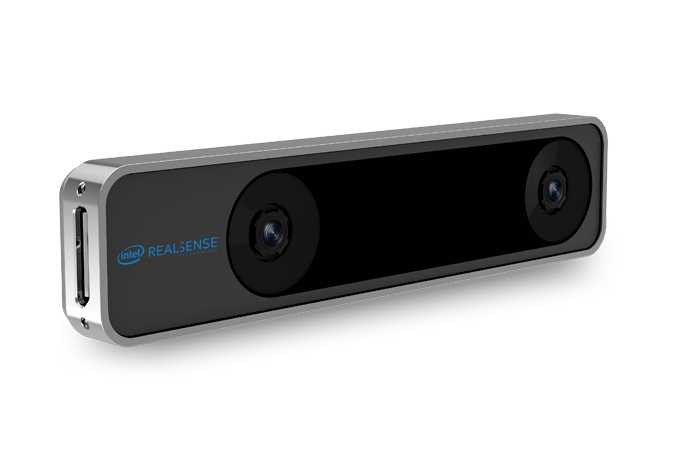
\includegraphics[width=\textwidth]{t265.png}
The camera our team used is the Intel Realsense T265; This camera makes use of it's binocular vision, in concordance with other sensors, such as it's built in IMU to provide a pose estimate within an inch of accuracy wihtout the use of enocder values. The camera's built in software uses advanced 'Simultaneous Localization and Mapping' algorithms, also know as V-SLAM algorithms, in order to make sense of this sensor data. Our code queries the pose estimate the camera provides, \textbf{allowing us to localize the robot even as it traverses over the barrier!}
\\
\\
In order to attain the camera's pose estimate we made use of a FTC Legal Java wrapper for the T265 software as the API provided by Intel is C++ exclusive. Our implementation is as follows:
\\

\begin{tcolorbox}
\textbf{Note:} After the class is constructed and the camera is initialized via the \textit{initializeT265} function, the \textit{updatePosition} function is called continuously every few milliseconds in the opMode, allowing for the translation values to stay accurate and provide real-time localization values as the robot is moving across the field. 
\end{tcolorbox}
\pagebreak
\inputminted[linenos, numbersep=5pt, tabsize=4, frame=lines, label=T265 Implementation, escapeinside=||,mathescape=true]{java}{{CodeFiles/T265_Code.java}}

\\
\noindent Although the T265 can be very useful at times, \textbf{we have faced a variety of challenges when using the camera.} One such challenge was the \textbf{lighting} of some tournament areas, leading to the V-SLAM algorithms becoming inconsistent leading to drift while traversing through the field. Another challenge we have experienced when using the camera is the \textbf{movement of other robots,} this is a prevalent problem as when the camera processes visual data, movement in the frame causes inaccuracies when calculating a position, as such, the repeated movement of several robots leads to further drift while moving in autonomous. To combat these problems we have implemented a custom odometry algorithm by making use of the encoders on our robot's drive motors. 
\\
\thispagestyle{empty}
\hspace{-0.65cm}\paragraph{Wheel Odometry}\mbox{} \\
To act as a supporting localization source to the T265 camera, our wheel odometry algorithm remains a reliable way to localize our robot. We make use of \textbf{encoders values} located on our robot's drive motors and apply several trigonometric formulas to convert these values into a robot pose. The mathematically process is detailed below.
\\ 
\\
Firstly we find the distance robot has traveled by converting the amount of ticks the left and right motors have travelled from the previously calculated position  and then converting this value into inches to find the total displacement in inches. This formula is applied to both wheels in order for the next step of the algorithm. This step is represented below:
\\
\\
\begin{equation*}
\Delta{tick} = tick' - tick
\end{equation*}
\begin{equation*}
D = 2\pi \cdot wheelRadius \cdot \frac{\Delta{tick}}{ticksPerRevolution}
\end{equation*}
\pagebreak
\\
 We then averaged the calculated inch displacement from the left and right wheels giving the overall displacement of the robot represented as D_c.
 
\begin{equation*}
D_c = \frac{D_l - D_r}{2}
\end{equation*}
\\
After attaining the current overall displacement we then break the overall displacement into the displacement of the $x$, $y$, and $\theta$ components by applying the trigonometric formulas detailed below. Finally we sum this this placement with the previously calculated components to attain the current position of the robot.
\begin{equation*}
x' = x + D_c \cdot \cos{x}
\end{equation*}
\begin{equation*}
y' = y + D_c \cdot \sin{y}
\end{equation*}
\begin{equation*}
\theta' = \theta + \frac{D_r - D_l}{L}
\end{equation*}
\\
This iterative process is implemented using the code below:
\inputminted[linenos, numbersep=5pt, tabsize=4, frame=lines, label=Odometry Pseudocode, escapeinside=||,mathescape=true]{java}{{CodeFiles/WheelOdometry.java}}


\thispagestyle{empty}
\subsubsection{Navigation PID}
In order to make use of our localization systems to move the robot, we make use of a PID controller, a feedback loop that uses the error in the current and destination positions of our robot in order to control our drive motors in such a way that our robot reaches the desired position. Although this concept seems abstract and complex it can be represented mathematically explained using the image below.
\begin{center}
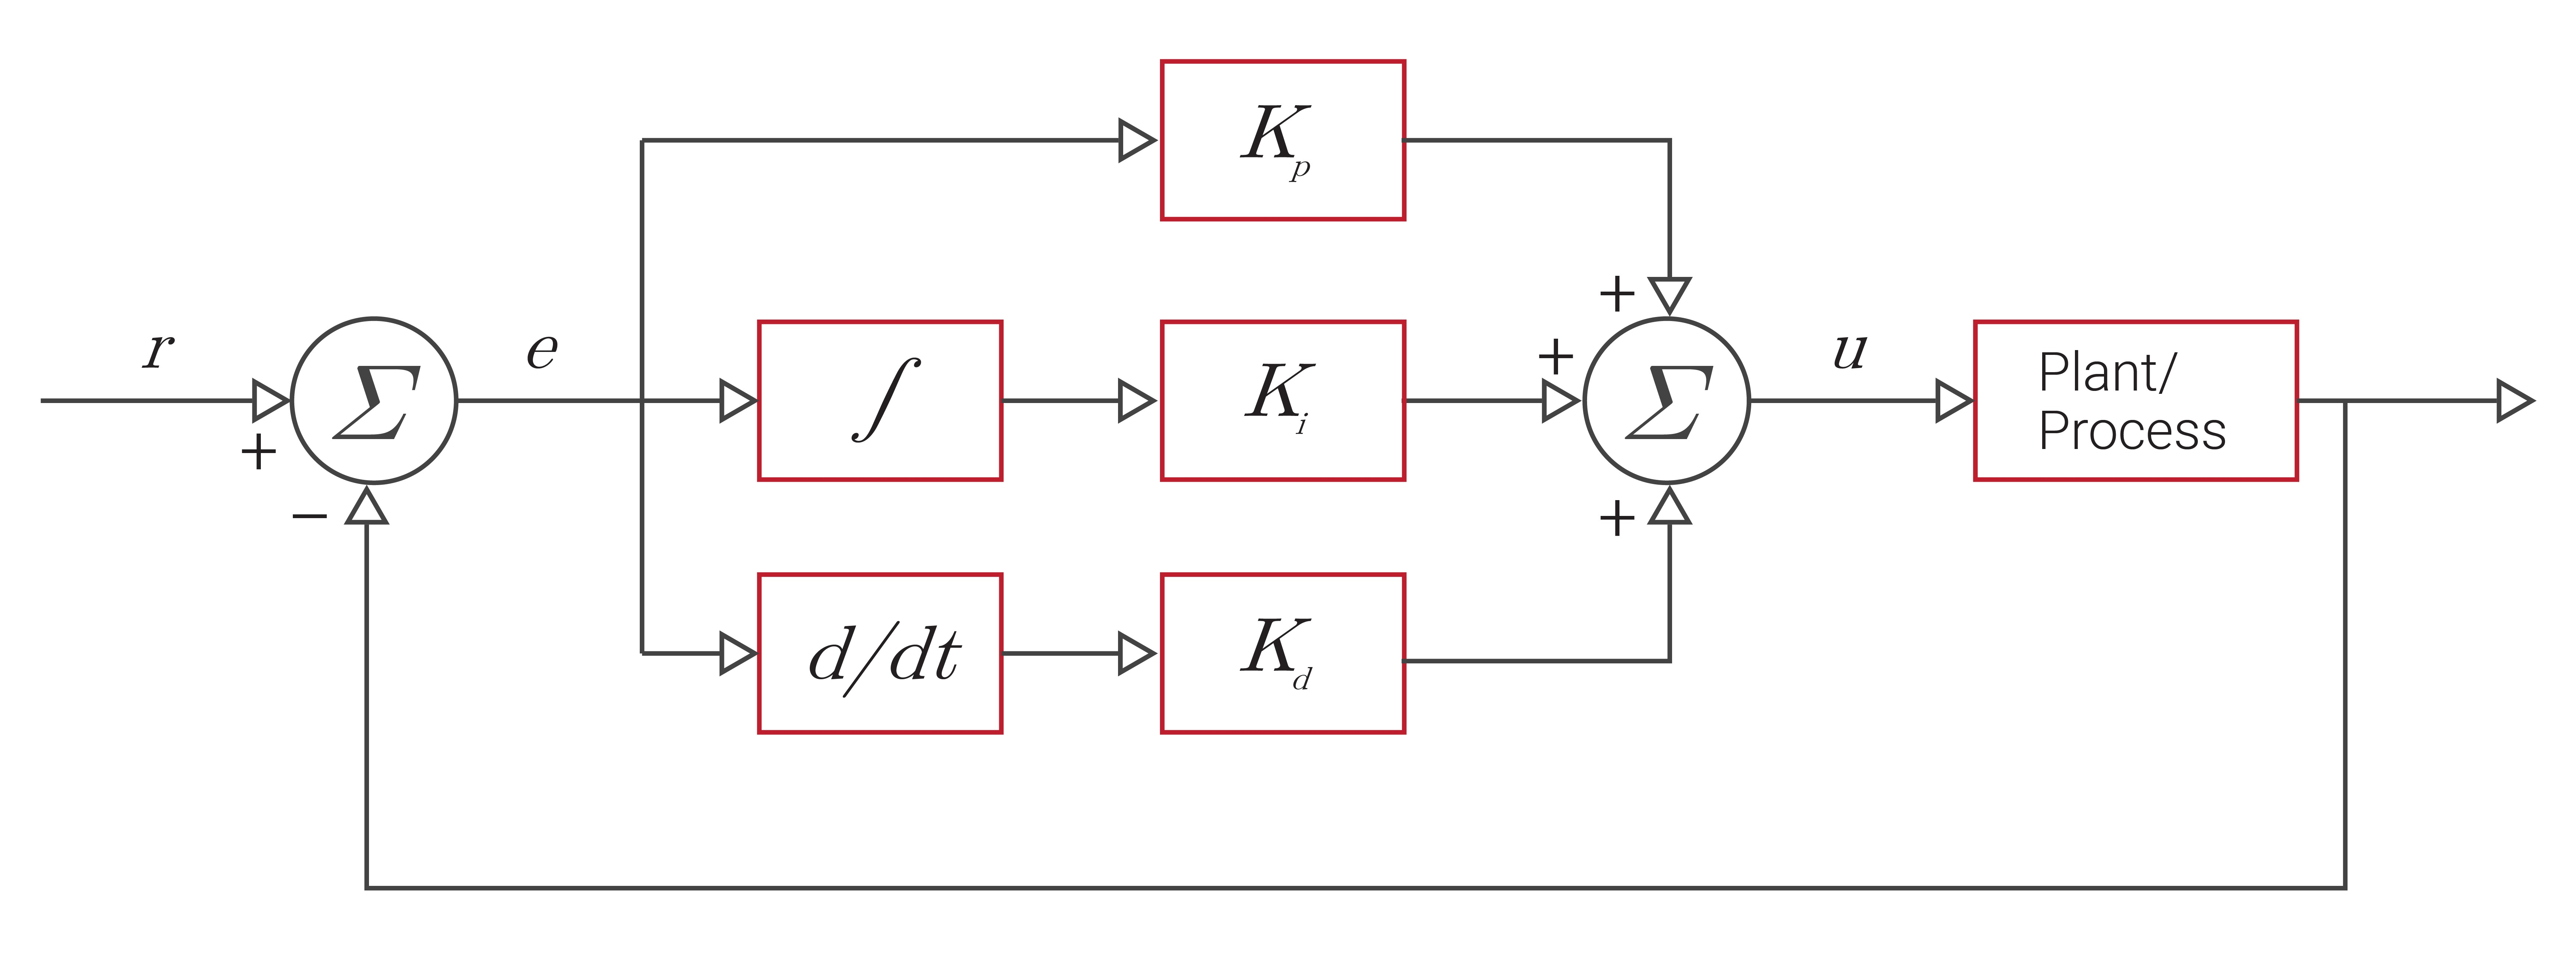
\includegraphics[width=\textwidth]{cnt_pid.jpg}
\end{center}


\noindent Essentially the equation for our PID controller contains three coefficients. $K_p$, $K_i$, and $K_d$. This first of these components is the proportional or $K_p$ component. This component of the equation is the primary driver of the navigation algorithm as we use the distance of the robot from it's target position and multiply it by the constant $K_p$ in order to set the appropriate powers to our motors; as the robot gets closer to the destination the powers the $K_p$ component outputs decreases until the robot oscillates around the target position.
\\ 
\\
After the robot oscillates around the destination position we then make use of the of the $K_d$ in order to dampen the rate of the robot as it arrives to its position. After testing, we decided against using the $K_i$ coefficient because we found that it did not affect the movement of our robot.
\newpage
\noindent Our navigation PID controller is implement below:

\inputminted[linenos, numbersep=5pt, tabsize=4, frame=lines, label=PID Implementation, escapeinside=||,mathescape=true]{java}{{CodeFiles/PID.java}}

\newpage
\thispagestyle{empty}
\subsubsection{Spline Paths}
This season we implemented a cubic spline interpolation program, which allows our robot to travel in a curved motion. After generating the spline curve we use our novel implementation of the pure pursuit algorithm to follow the points along the curve in a smooth manner. This has allowed us to \textbf{pursue smooth and efficient autonomous paths} and \textbf{accounts for the lack of strafing capability of our tank style drive train}.

\hspace{-0.65cm}\paragraph{Path Generation}\mbox{}\\
 Firstly after giving the generation program a series of points, it creates a series of cubic, peicewise functions, one between each point given, giving a total of $n-1$ points where $n$ is the number of points inputted. The general format of the series of equations are mathematically provided below:
\begin{equation}
    f\left(x\right)=\begin{cases} 
a_1x^3+b_1x^2+c_1x+d_1&\text{if }x\in\left[x_1,x_2\right]\\ 
a_2x^3+b_2x^2+c_2x+d_2&\text{if }x\in\left(x_2,x_3\right]\\ 
\dots\\ 
a_nx^3+b_nx^2+c_nx+d_n&\text{if }x\in\left(x_{n},x_{n+1}\right]\,. 
\end{cases}
\end{equation}
\\
We then combine each of the equations between the points to provide a smooth curve. An example of the program output using a series of sample points with along with the newly generated curve is shown graphically below:
\\
\\
\begin{center}

\begin{tikzpicture}

		\pgfplotsset{
			scale only axis,
		}

		\begin{axis}[
			xlabel=$x$,
			ylabel=$y$,
			samples=100,
			]\addplot [only marks] table {
-1.5 -1.2
-.2 0
1 0.5
5 1
10 1.2
15 2
20 1
};
		\end{axis}
		
				\pgfplotsset{
			scale only axis,
		}

		\begin{axis}[
			xlabel=$x$,
			ylabel=$y$,
			samples=100,
			]\addplot [only marks] table {
-1.5 -1.2
-0.2 0
1 0.5
5 1
10 1.2
15 2
20 1
};
			
			\addplot[][domain=-1.5:-0.2]{+-0.07516004606833009*x^3+-0.3382202073074854*x^2+0.5427670899711728*x^1+0.12148094591798733*x^0};

			\addplot[][domain=-0.2:1]{+0.06901369090311398*x^3+-0.25171596512461897*x^2+0.560067938407746*x^1+0.12263433581375889*x^0};

			\addplot[][domain=1:5]{+0.0025014055495786265*x^3+-0.05217910906401291*x^2+0.36053108234714004*x^1+0.18914662116729425*x^0};

			\addplot[][domain=5:10]{+0.0034777888470503854*x^3+-0.0668248585260893*x^2+0.43375982965752197*x^1+0.06709870898332437*x^0};

			\addplot[][domain=10:15]{+-0.006725733907118523*x^3+0.23928082409897794*x^2+-2.6272969965931505*x^1+10.270621463152233*x^0};

			\addplot[][domain=15:20]{+0.004225146781423704*x^3+-0.25350880688542227*x^2+4.764547468172853*x^1+-26.688600860677784*x^0};
		\end{axis}

\end{tikzpicture}
  $\mathcal{D}=\left\{ \left(-1.5,-1.2\right),\left(-.2,0\right),\left(1,.5\right),\left(5,1\right),\left(10,1.2\right),\left(15,2\right),\left(20,1\right)\right\}$
\end{center}

\begin{center}
  
\end{center}


\noindent To compute the coefficients of each equation. We must create separate polynomials for each pair of points such that the first and second derivative of all polynomials are identical in the points where they touch their adjacent polynomial. This is done using a iterative process which is displayed by our code below:
\\
\\
\inputminted[linenos, numbersep=5pt, tabsize=4, frame=lines, label=Spline Interpolator, escapeinside=||,mathescape=true]{java}{{CodeFiles/SplineGen.java}}
\\ 



\newpage
\thispagestyle{empty}


\section{Vision}
This season, at the beginning of the autonomous period we need to determine which of three bar-code positions that our team shipping element is placed at. In order to determine this, we use a custom-made Vuforia algorithm. Our algorithm creates a rectangular box on all three possible positions of the shipping element and then takes the average red, green, or blue values of each barcode, returning the box which matches the RGB value of our shipping element the best.
\subsection{Image Segmentation}
Firstly our algorithm takes three pixel "boxes" from our image. It then segments these boxes into a grid of RGB values for processing. Take a look at our segmentation algorithm, highlighting these boxes below:
\\
\\
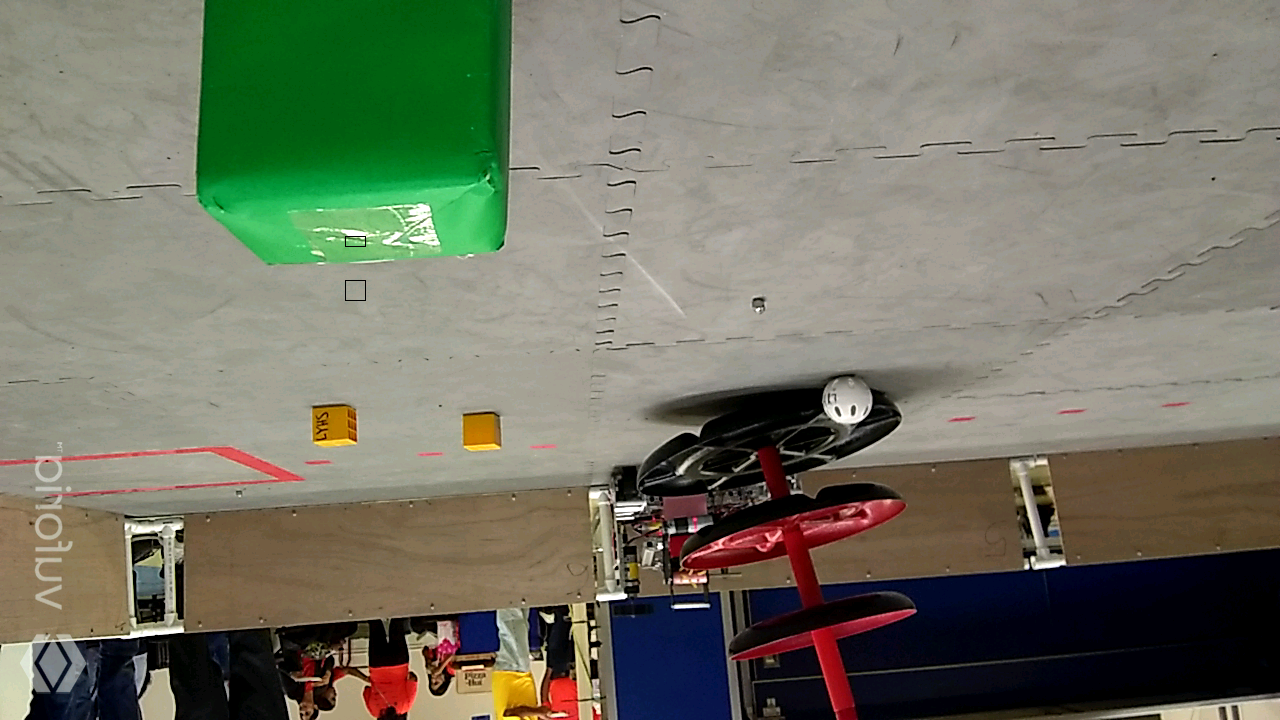
\includegraphics[width=\textwidth]{Vuforia_Segmentation.png}
\\
\\
The Vuforia engine streamlines this process, as when the image is taken Vuforia automatically returns a grid of RGB values, therefore all we need to do is define the bounds for these rectangles. 
\\
\inputminted[linenos, numbersep=5pt, tabsize=4, frame=lines, label=Image Segmentation, escapeinside=||,mathescape=true]{java}{{CodeFiles/Vuforia1.java}}

\subsection{Object Detection}
\\ 
After attaining a way to take and process the image, we will now cover the actual algorithm. Firstly after defining the bounds of the tree rectangles, with each reading the center of the barcode, we take the average green intensity values of these spots. We then compare the averages and return the square which has the highest green intensity. This algorithm is implemented below. \\ 
\inputminted[linenos, numbersep=5pt, tabsize=4, frame=lines, label=Image Segmentation, escapeinside=||,mathescape=true]{java}{{CodeFiles/Vuforia2.java}}



\newpage
\thispagestyle{empty}
%\subsection{Vuforia}
\newpage
\thispagestyle{empty}
\section{Tele-OP Automation}
At the moment we have implemented several small automations in our tele-op programs in order to boost our driver's overall performance while still giving them the freedom to maneuver the individual modules as they please. 
\subsection{Arm Control}
One of our noteable automations is our arm controller. We have made use of the built in PID controller that the SDK provides to allow our drivers to rise and lower the arm automatically to the high and sweeping positions at the press of a button. 
\subsection{Carousel Control}

\subsection{Drive Control}

\newpage
\thispagestyle{empty}

\section{Autonomous Strategy}
\subsection{Diagram}
\begin{center}
\begin{tikzpicture}[node distance=2cm, auto]
<TikZ code>
\node (start) [startstop] {Start};
\node (in1) [io, below of=start] {Read Shipping Element Position};
\node (pro1) [process, below of=in1] {Navigate to Shipping Hub};
\node (dec1) [decision, below of=pro1, yshift=-1cm] {Element Position};
\node (pro2a) [process, below of=dec1, yshift=-1cm] {Drop Middle};
\node (pro2b) [process, below of=dec1, yshift=-1cm, xshift=4cm] {Drop Bottom};
\node (pro2c) [process, below of=dec1, yshift=-1cm, xshift=-4cm] {Drop Top};
\node (out1) [io, below of=pro2a] {Navigate to Carousel};
\node (pro3a) [process, below of=out1] {Spin Carousel};
\node (stop) [startstop, below of=pro3a] {Park};

\draw [arrow] (start) -- (in1);
\draw [arrow] (in1) -- (pro1);
\draw [arrow] (pro1) -- (dec1);
\draw [arrow] (dec1) -- (pro2a);
\draw [arrow] (dec1) -- (pro2b);
\draw [arrow] (pro2c) -- (out1);
\draw [arrow] (pro2a) -- (out1);
\draw [arrow] (pro2b) -- (out1);
\draw [arrow] (dec1) -- (pro2c);
\draw [arrow] (out1) -- (pro3a);
\draw [arrow] (pro3a) -- (stop);

\end{tikzpicture}
\end{center}

 

\end{document}